\documentclass[1p]{elsarticle_modified}
%\bibliographystyle{elsarticle-num}

%\usepackage[colorlinks]{hyperref}
%\usepackage{abbrmath_seonhwa} %\Abb, \Ascr, \Acal ,\Abf, \Afrak
\usepackage{amsfonts}
\usepackage{amssymb}
\usepackage{amsmath}
\usepackage{amsthm}
\usepackage{scalefnt}
\usepackage{amsbsy}
\usepackage{kotex}
\usepackage{caption}
\usepackage{subfig}
\usepackage{color}
\usepackage{graphicx}
\usepackage{xcolor} %% white, black, red, green, blue, cyan, magenta, yellow
\usepackage{float}
\usepackage{setspace}
\usepackage{hyperref}

\usepackage{tikz}
\usetikzlibrary{arrows}

\usepackage{multirow}
\usepackage{array} % fixed length table
\usepackage{hhline}

%%%%%%%%%%%%%%%%%%%%%
\makeatletter
\renewcommand*\env@matrix[1][\arraystretch]{%
	\edef\arraystretch{#1}%
	\hskip -\arraycolsep
	\let\@ifnextchar\new@ifnextchar
	\array{*\c@MaxMatrixCols c}}
\makeatother %https://tex.stackexchange.com/questions/14071/how-can-i-increase-the-line-spacing-in-a-matrix
%%%%%%%%%%%%%%%

\usepackage[normalem]{ulem}

\newcommand{\msout}[1]{\ifmmode\text{\sout{\ensuremath{#1}}}\else\sout{#1}\fi}
%SOURCE: \msout is \stkout macro in https://tex.stackexchange.com/questions/20609/strikeout-in-math-mode

\newcommand{\cancel}[1]{
	\ifmmode
	{\color{red}\msout{#1}}
	\else
	{\color{red}\sout{#1}}
	\fi
}

\newcommand{\add}[1]{
	{\color{blue}\uwave{#1}}
}

\newcommand{\replace}[2]{
	\ifmmode
	{\color{red}\msout{#1}}{\color{blue}\uwave{#2}}
	\else
	{\color{red}\sout{#1}}{\color{blue}\uwave{#2}}
	\fi
}

\newcommand{\Sol}{\mathcal{S}} %segment
\newcommand{\D}{D} %diagram
\newcommand{\A}{\mathcal{A}} %arc


%%%%%%%%%%%%%%%%%%%%%%%%%%%%%5 test

\def\sl{\operatorname{\textup{SL}}(2,\Cbb)}
\def\psl{\operatorname{\textup{PSL}}(2,\Cbb)}
\def\quan{\mkern 1mu \triangleright \mkern 1mu}

\theoremstyle{definition}
\newtheorem{thm}{Theorem}[section]
\newtheorem{prop}[thm]{Proposition}
\newtheorem{lem}[thm]{Lemma}
\newtheorem{ques}[thm]{Question}
\newtheorem{cor}[thm]{Corollary}
\newtheorem{defn}[thm]{Definition}
\newtheorem{exam}[thm]{Example}
\newtheorem{rmk}[thm]{Remark}
\newtheorem{alg}[thm]{Algorithm}

\newcommand{\I}{\sqrt{-1}}
\begin{document}

%\begin{frontmatter}
%
%\title{Boundary parabolic representations of knots up to 8 crossings}
%
%%% Group authors per affiliation:
%\author{Yunhi Cho} 
%\address{Department of Mathematics, University of Seoul, Seoul, Korea}
%\ead{yhcho@uos.ac.kr}
%
%
%\author{Seonhwa Kim} %\fnref{s_kim}}
%\address{Center for Geometry and Physics, Institute for Basic Science, Pohang, 37673, Korea}
%\ead{ryeona17@ibs.re.kr}
%
%\author{Hyuk Kim}
%\address{Department of Mathematical Sciences, Seoul National University, Seoul 08826, Korea}
%\ead{hyukkim@snu.ac.kr}
%
%\author{Seokbeom Yoon}
%\address{Department of Mathematical Sciences, Seoul National University, Seoul, 08826,  Korea}
%\ead{sbyoon15@snu.ac.kr}
%
%\begin{abstract}
%We find all boundary parabolic representation of knots up to 8 crossings.
%
%\end{abstract}
%\begin{keyword}
%    \MSC[2010] 57M25 
%\end{keyword}
%
%\end{frontmatter}

%\linenumbers
%\tableofcontents
%
\newcommand\colored[1]{\textcolor{white}{\rule[-0.35ex]{0.8em}{1.4ex}}\kern-0.8em\color{red} #1}%
%\newcommand\colored[1]{\textcolor{white}{ #1}\kern-2.17ex	\textcolor{white}{ #1}\kern-1.81ex	\textcolor{white}{ #1}\kern-2.15ex\color{red}#1	}

{\Large $\underline{12a_{0527}~(K12a_{0527})}$}

\setlength{\tabcolsep}{10pt}
\renewcommand{\arraystretch}{1.6}
\vspace{1cm}\begin{tabular}{m{100pt}>{\centering\arraybackslash}m{274pt}}
\multirow{5}{120pt}{
	\centering
	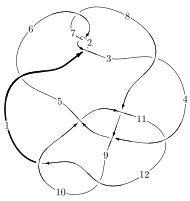
\includegraphics[width=112pt]{../../../GIT/diagram.site/Diagrams/png/1328_12a_0527.png}\\
\ \ \ A knot diagram\footnotemark}&
\allowdisplaybreaks
\textbf{Linearized knot diagam} \\
\cline{2-2}
 &
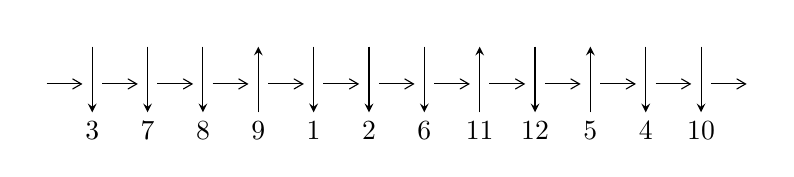
\begin{tikzpicture}[x=20pt, y=17pt]
	% nodes
	\node (C0) at (0, 0) {};
	\node (C1) at (1, 0) {};
	\node (C1U) at (1, +1) {};
	\node (C1D) at (1, -1) {3};

	\node (C2) at (2, 0) {};
	\node (C2U) at (2, +1) {};
	\node (C2D) at (2, -1) {7};

	\node (C3) at (3, 0) {};
	\node (C3U) at (3, +1) {};
	\node (C3D) at (3, -1) {8};

	\node (C4) at (4, 0) {};
	\node (C4U) at (4, +1) {};
	\node (C4D) at (4, -1) {9};

	\node (C5) at (5, 0) {};
	\node (C5U) at (5, +1) {};
	\node (C5D) at (5, -1) {1};

	\node (C6) at (6, 0) {};
	\node (C6U) at (6, +1) {};
	\node (C6D) at (6, -1) {2};

	\node (C7) at (7, 0) {};
	\node (C7U) at (7, +1) {};
	\node (C7D) at (7, -1) {6};

	\node (C8) at (8, 0) {};
	\node (C8U) at (8, +1) {};
	\node (C8D) at (8, -1) {11};

	\node (C9) at (9, 0) {};
	\node (C9U) at (9, +1) {};
	\node (C9D) at (9, -1) {12};

	\node (C10) at (10, 0) {};
	\node (C10U) at (10, +1) {};
	\node (C10D) at (10, -1) {5};

	\node (C11) at (11, 0) {};
	\node (C11U) at (11, +1) {};
	\node (C11D) at (11, -1) {4};

	\node (C12) at (12, 0) {};
	\node (C12U) at (12, +1) {};
	\node (C12D) at (12, -1) {10};
	\node (C13) at (13, 0) {};

	% arrows
	\draw[->,>={angle 60}]
	(C0) edge (C1) (C1) edge (C2) (C2) edge (C3) (C3) edge (C4) (C4) edge (C5) (C5) edge (C6) (C6) edge (C7) (C7) edge (C8) (C8) edge (C9) (C9) edge (C10) (C10) edge (C11) (C11) edge (C12) (C12) edge (C13) ;	\draw[->,>=stealth]
	(C1U) edge (C1D) (C2U) edge (C2D) (C3U) edge (C3D) (C4D) edge (C4U) (C5U) edge (C5D) (C6U) edge (C6D) (C7U) edge (C7D) (C8D) edge (C8U) (C9U) edge (C9D) (C10D) edge (C10U) (C11U) edge (C11D) (C12U) edge (C12D) ;
	\end{tikzpicture} \\
\hhline{~~} \\& 
\textbf{Solving Sequence} \\ \cline{2-2} 
 &
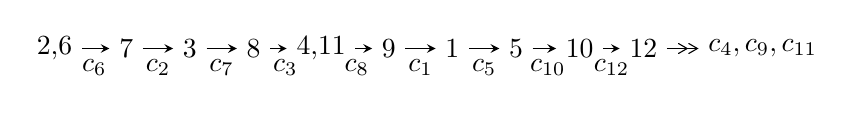
\begin{tikzpicture}[x=23pt, y=7pt]
	% node
	\node (A0) at (-1/8, 0) {2,6};
	\node (A1) at (1, 0) {7};
	\node (A2) at (2, 0) {3};
	\node (A3) at (3, 0) {8};
	\node (A4) at (65/16, 0) {4,11};
	\node (A5) at (41/8, 0) {9};
	\node (A6) at (49/8, 0) {1};
	\node (A7) at (57/8, 0) {5};
	\node (A8) at (65/8, 0) {10};
	\node (A9) at (73/8, 0) {12};
	\node (C1) at (1/2, -1) {$c_{6}$};
	\node (C2) at (3/2, -1) {$c_{2}$};
	\node (C3) at (5/2, -1) {$c_{7}$};
	\node (C4) at (7/2, -1) {$c_{3}$};
	\node (C5) at (37/8, -1) {$c_{8}$};
	\node (C6) at (45/8, -1) {$c_{1}$};
	\node (C7) at (53/8, -1) {$c_{5}$};
	\node (C8) at (61/8, -1) {$c_{10}$};
	\node (C9) at (69/8, -1) {$c_{12}$};
	\node (A10) at (11, 0) {$c_{4},c_{9},c_{11}$};

	% edge
	\draw[->,>=stealth]	
	(A0) edge (A1) (A1) edge (A2) (A2) edge (A3) (A3) edge (A4) (A4) edge (A5) (A5) edge (A6) (A6) edge (A7) (A7) edge (A8) (A8) edge (A9) ;
	\draw[->>,>={angle 60}]	
	(A9) edge (A10);
\end{tikzpicture} \\ 

\end{tabular} \\

\footnotetext{
The image of knot diagram is generated by the software ``\textbf{Draw programme}" developed by Andrew Bartholomew(\url{http://www.layer8.co.uk/maths/draw/index.htm\#Running-draw}), where we modified some parts for our purpose(\url{https://github.com/CATsTAILs/LinksPainter}).
}\phantom \\ \newline 
\centering \textbf{Ideals for irreducible components\footnotemark of $X_{\text{par}}$} 
 
\begin{align*}
I^u_{1}&=\langle 
-2.62656\times10^{32} u^{100}-1.37621\times10^{32} u^{99}+\cdots+1.43355\times10^{32} b-4.87406\times10^{32},\\
\phantom{I^u_{1}}&\phantom{= \langle  }7.89761\times10^{32} u^{100}-1.36318\times10^{33} u^{99}+\cdots+1.43355\times10^{32} a+6.41450\times10^{32},\;u^{101}-2 u^{100}+\cdots-3 u-1\rangle \\
I^u_{2}&=\langle 
b+u-1,\;- u^2+a+u,\;u^3- u^2+1\rangle \\
\\
\end{align*}
\raggedright * 2 irreducible components of $\dim_{\mathbb{C}}=0$, with total 104 representations.\\
\footnotetext{All coefficients of polynomials are rational numbers. But the coefficients are sometimes approximated in decimal forms when there is not enough margin.}
\newpage
\renewcommand{\arraystretch}{1}
\centering \section*{I. $I^u_{1}= \langle -2.63\times10^{32} u^{100}-1.38\times10^{32} u^{99}+\cdots+1.43\times10^{32} b-4.87\times10^{32},\;7.90\times10^{32} u^{100}-1.36\times10^{33} u^{99}+\cdots+1.43\times10^{32} a+6.41\times10^{32},\;u^{101}-2 u^{100}+\cdots-3 u-1 \rangle$}
\flushleft \textbf{(i) Arc colorings}\\
\begin{tabular}{m{7pt} m{180pt} m{7pt} m{180pt} }
\flushright $a_{2}=$&$\begin{pmatrix}0\\u\end{pmatrix}$ \\
\flushright $a_{6}=$&$\begin{pmatrix}1\\0\end{pmatrix}$ \\
\flushright $a_{7}=$&$\begin{pmatrix}1\\u^2\end{pmatrix}$ \\
\flushright $a_{3}=$&$\begin{pmatrix}- u\\- u^3+u\end{pmatrix}$ \\
\flushright $a_{8}=$&$\begin{pmatrix}- u^2+1\\u^2\end{pmatrix}$ \\
\flushright $a_{4}=$&$\begin{pmatrix}u^7-2 u^5+2 u^3-2 u\\- u^7+u^5-2 u^3+u\end{pmatrix}$ \\
\flushright $a_{11}=$&$\begin{pmatrix}-5.50914 u^{100}+9.50914 u^{99}+\cdots-11.1589 u-4.47457\\1.83221 u^{100}+0.960001 u^{99}+\cdots+8.36542 u+3.40000\end{pmatrix}$ \\
\flushright $a_{9}=$&$\begin{pmatrix}1.84477 u^{100}-2.24477 u^{99}+\cdots+5.88323 u+0.722386\\-0.602902 u^{100}+0.200001 u^{99}+\cdots-0.0776162 u-0.400001\end{pmatrix}$ \\
\flushright $a_{1}=$&$\begin{pmatrix}u^3\\u^5- u^3+u\end{pmatrix}$ \\
\flushright $a_{5}=$&$\begin{pmatrix}- u^8+u^6- u^4+1\\- u^{10}+2 u^8-3 u^6+2 u^4- u^2\end{pmatrix}$ \\
\flushright $a_{10}=$&$\begin{pmatrix}-4.64586 u^{100}+6.04586 u^{99}+\cdots-15.4372 u-6.42293\\0.439796 u^{100}+2.56000 u^{99}+\cdots+8.01707 u+3.60000\end{pmatrix}$ \\
\flushright $a_{12}=$&$\begin{pmatrix}-4.18435 u^{100}+5.38435 u^{99}+\cdots-13.0030 u-6.29217\\0.241103 u^{100}+2.56000 u^{99}+\cdots+8.34783 u+3.40000\end{pmatrix}$\\&\end{tabular}
\flushleft \textbf{(ii) Obstruction class $= -1$}\\~\\
\flushleft \textbf{(iii) Cusp Shapes $= -31.9407 u^{100}+84.2414 u^{99}+\cdots+10.3636 u+24.0193$}\\~\\
\newpage\renewcommand{\arraystretch}{1}
\flushleft \textbf{(iv) u-Polynomials at the component}\newline \\
\begin{tabular}{m{50pt}|m{274pt}}
Crossings & \hspace{64pt}u-Polynomials at each crossing \\
\hline $$\begin{aligned}c_{1},c_{7}\end{aligned}$$&$\begin{aligned}
&u^{101}+36 u^{100}+\cdots+u+1
\end{aligned}$\\
\hline $$\begin{aligned}c_{2},c_{6}\end{aligned}$$&$\begin{aligned}
&u^{101}-2 u^{100}+\cdots-3 u-1
\end{aligned}$\\
\hline $$\begin{aligned}c_{3},c_{5}\end{aligned}$$&$\begin{aligned}
&u^{101}+2 u^{100}+\cdots-31477 u-8353
\end{aligned}$\\
\hline $$\begin{aligned}c_{4}\end{aligned}$$&$\begin{aligned}
&u^{101}-2 u^{100}+\cdots+u-1
\end{aligned}$\\
\hline $$\begin{aligned}c_{8}\end{aligned}$$&$\begin{aligned}
&u^{101}+17 u^{100}+\cdots+4 u-8
\end{aligned}$\\
\hline $$\begin{aligned}c_{9},c_{12}\end{aligned}$$&$\begin{aligned}
&u^{101}-4 u^{100}+\cdots-2 u-1
\end{aligned}$\\
\hline $$\begin{aligned}c_{10}\end{aligned}$$&$\begin{aligned}
&u^{101}- u^{100}+\cdots-2263262 u-275501
\end{aligned}$\\
\hline $$\begin{aligned}c_{11}\end{aligned}$$&$\begin{aligned}
&u^{101}+u^{100}+\cdots-9608 u-3329
\end{aligned}$\\
\hline
\end{tabular}\\~\\
\newpage\renewcommand{\arraystretch}{1}
\flushleft \textbf{(v) Riley Polynomials at the component}\newline \\
\begin{tabular}{m{50pt}|m{274pt}}
Crossings & \hspace{64pt}Riley Polynomials at each crossing \\
\hline $$\begin{aligned}c_{1},c_{7}\end{aligned}$$&$\begin{aligned}
&y^{101}+60 y^{100}+\cdots-215 y-1
\end{aligned}$\\
\hline $$\begin{aligned}c_{2},c_{6}\end{aligned}$$&$\begin{aligned}
&y^{101}-36 y^{100}+\cdots+y-1
\end{aligned}$\\
\hline $$\begin{aligned}c_{3},c_{5}\end{aligned}$$&$\begin{aligned}
&y^{101}-84 y^{100}+\cdots+315879129 y-69772609
\end{aligned}$\\
\hline $$\begin{aligned}c_{4}\end{aligned}$$&$\begin{aligned}
&y^{101}+20 y^{100}+\cdots+y-1
\end{aligned}$\\
\hline $$\begin{aligned}c_{8}\end{aligned}$$&$\begin{aligned}
&y^{101}+21 y^{100}+\cdots+80 y-64
\end{aligned}$\\
\hline $$\begin{aligned}c_{9},c_{12}\end{aligned}$$&$\begin{aligned}
&y^{101}-78 y^{100}+\cdots+142 y-1
\end{aligned}$\\
\hline $$\begin{aligned}c_{10}\end{aligned}$$&$\begin{aligned}
&y^{101}-53 y^{100}+\cdots-5937265797024 y-75900801001
\end{aligned}$\\
\hline $$\begin{aligned}c_{11}\end{aligned}$$&$\begin{aligned}
&y^{101}-129 y^{100}+\cdots+336808740 y-11082241
\end{aligned}$\\
\hline
\end{tabular}\\~\\
\newpage\flushleft \textbf{(vi) Complex Volumes and Cusp Shapes}
$$\begin{array}{c|c|c}  
\text{Solutions to }I^u_{1}& \I (\text{vol} + \sqrt{-1}CS) & \text{Cusp shape}\\
 \hline 
\begin{aligned}
u &= \phantom{-}0.580578 + 0.817482 I \\
a &= \phantom{-}1.08176 + 2.75518 I \\
b &= -1.61602 - 1.97604 I\end{aligned}
 & -6.13347 + 12.43020 I & \phantom{-0.000000 } 0 \\ \hline\begin{aligned}
u &= \phantom{-}0.580578 - 0.817482 I \\
a &= \phantom{-}1.08176 - 2.75518 I \\
b &= -1.61602 + 1.97604 I\end{aligned}
 & -6.13347 - 12.43020 I & \phantom{-0.000000 } 0 \\ \hline\begin{aligned}
u &= -0.776866 + 0.636255 I \\
a &= -1.285090 - 0.032532 I \\
b &= -0.235532 + 0.454753 I\end{aligned}
 & -0.351074 - 0.411440 I & \phantom{-0.000000 } 0 \\ \hline\begin{aligned}
u &= -0.776866 - 0.636255 I \\
a &= -1.285090 + 0.032532 I \\
b &= -0.235532 - 0.454753 I\end{aligned}
 & -0.351074 + 0.411440 I & \phantom{-0.000000 } 0 \\ \hline\begin{aligned}
u &= -0.579941 + 0.831261 I \\
a &= -0.20262 + 1.51768 I \\
b &= \phantom{-}0.491882 - 1.239610 I\end{aligned}
 & -5.31423 - 4.01863 I & \phantom{-0.000000 } 0 \\ \hline\begin{aligned}
u &= -0.579941 - 0.831261 I \\
a &= -0.20262 - 1.51768 I \\
b &= \phantom{-}0.491882 + 1.239610 I\end{aligned}
 & -5.31423 + 4.01863 I & \phantom{-0.000000 } 0 \\ \hline\begin{aligned}
u &= \phantom{-}0.731897 + 0.717631 I \\
a &= -0.985525 - 0.373921 I \\
b &= \phantom{-}1.232150 + 0.021103 I\end{aligned}
 & \phantom{-}3.54399 - 0.83039 I & \phantom{-0.000000 } 0 \\ \hline\begin{aligned}
u &= \phantom{-}0.731897 - 0.717631 I \\
a &= -0.985525 + 0.373921 I \\
b &= \phantom{-}1.232150 - 0.021103 I\end{aligned}
 & \phantom{-}3.54399 + 0.83039 I & \phantom{-0.000000 } 0 \\ \hline\begin{aligned}
u &= \phantom{-}0.579045 + 0.782616 I \\
a &= -1.41006 - 2.92308 I \\
b &= \phantom{-}1.80130 + 2.00177 I\end{aligned}
 & -1.15835 + 6.39204 I & \phantom{-0.000000 } 0 \\ \hline\begin{aligned}
u &= \phantom{-}0.579045 - 0.782616 I \\
a &= -1.41006 + 2.92308 I \\
b &= \phantom{-}1.80130 - 2.00177 I\end{aligned}
 & -1.15835 - 6.39204 I & \phantom{-0.000000 } 0\\
 \hline 
 \end{array}$$\newpage$$\begin{array}{c|c|c}  
\text{Solutions to }I^u_{1}& \I (\text{vol} + \sqrt{-1}CS) & \text{Cusp shape}\\
 \hline 
\begin{aligned}
u &= \phantom{-}0.992696 + 0.288852 I \\
a &= -0.413171 - 1.163250 I \\
b &= \phantom{-}0.357560 - 0.746316 I\end{aligned}
 & -5.66355 - 7.67808 I & \phantom{-0.000000 } 0 \\ \hline\begin{aligned}
u &= \phantom{-}0.992696 - 0.288852 I \\
a &= -0.413171 + 1.163250 I \\
b &= \phantom{-}0.357560 + 0.746316 I\end{aligned}
 & -5.66355 + 7.67808 I & \phantom{-0.000000 } 0 \\ \hline\begin{aligned}
u &= -0.586808 + 0.759798 I \\
a &= \phantom{-}0.04149 - 2.11805 I \\
b &= -0.78617 + 1.40337 I\end{aligned}
 & -1.12071 - 2.11881 I & \phantom{-0.000000 } 0 \\ \hline\begin{aligned}
u &= -0.586808 - 0.759798 I \\
a &= \phantom{-}0.04149 + 2.11805 I \\
b &= -0.78617 - 1.40337 I\end{aligned}
 & -1.12071 + 2.11881 I & \phantom{-0.000000 } 0 \\ \hline\begin{aligned}
u &= \phantom{-}0.551923 + 0.766712 I \\
a &= \phantom{-}1.00983 - 2.09875 I \\
b &= -0.93227 + 1.55605 I\end{aligned}
 & -5.52348 + 3.44945 I & \phantom{-0.000000 } 0 \\ \hline\begin{aligned}
u &= \phantom{-}0.551923 - 0.766712 I \\
a &= \phantom{-}1.00983 + 2.09875 I \\
b &= -0.93227 - 1.55605 I\end{aligned}
 & -5.52348 - 3.44945 I & \phantom{-0.000000 } 0 \\ \hline\begin{aligned}
u &= -0.999347 + 0.340848 I \\
a &= \phantom{-}1.060780 - 0.155870 I \\
b &= \phantom{-}0.171910 - 0.581163 I\end{aligned}
 & -5.38574 - 1.49082 I & \phantom{-0.000000 } 0 \\ \hline\begin{aligned}
u &= -0.999347 - 0.340848 I \\
a &= \phantom{-}1.060780 + 0.155870 I \\
b &= \phantom{-}0.171910 + 0.581163 I\end{aligned}
 & -5.38574 + 1.49082 I & \phantom{-0.000000 } 0 \\ \hline\begin{aligned}
u &= -0.867440 + 0.602442 I \\
a &= -1.027350 - 0.522687 I \\
b &= -0.41382 + 1.88947 I\end{aligned}
 & -2.06528 + 2.36638 I & \phantom{-0.000000 } 0 \\ \hline\begin{aligned}
u &= -0.867440 - 0.602442 I \\
a &= -1.027350 + 0.522687 I \\
b &= -0.41382 - 1.88947 I\end{aligned}
 & -2.06528 - 2.36638 I & \phantom{-0.000000 } 0\\
 \hline 
 \end{array}$$\newpage$$\begin{array}{c|c|c}  
\text{Solutions to }I^u_{1}& \I (\text{vol} + \sqrt{-1}CS) & \text{Cusp shape}\\
 \hline 
\begin{aligned}
u &= \phantom{-}0.830410 + 0.659590 I \\
a &= \phantom{-}3.26701 + 2.72075 I \\
b &= -3.24052 + 0.35453 I\end{aligned}
 & \phantom{-}0.66876 - 2.15524 I & \phantom{-0.000000 } 0 \\ \hline\begin{aligned}
u &= \phantom{-}0.830410 - 0.659590 I \\
a &= \phantom{-}3.26701 - 2.72075 I \\
b &= -3.24052 - 0.35453 I\end{aligned}
 & \phantom{-}0.66876 + 2.15524 I & \phantom{-0.000000 } 0 \\ \hline\begin{aligned}
u &= -0.790678 + 0.720657 I \\
a &= \phantom{-}0.373565 + 0.794306 I \\
b &= \phantom{-}0.26102 - 1.55215 I\end{aligned}
 & \phantom{-}4.26660 - 1.41032 I & \phantom{-0.000000 } 0 \\ \hline\begin{aligned}
u &= -0.790678 - 0.720657 I \\
a &= \phantom{-}0.373565 - 0.794306 I \\
b &= \phantom{-}0.26102 + 1.55215 I\end{aligned}
 & \phantom{-}4.26660 + 1.41032 I & \phantom{-0.000000 } 0 \\ \hline\begin{aligned}
u &= -0.557322 + 0.741721 I \\
a &= \phantom{-}2.71247 + 1.31477 I \\
b &= -0.38069 - 1.74543 I\end{aligned}
 & -3.15042 - 1.23136 I & \phantom{-0.000000 } 0 \\ \hline\begin{aligned}
u &= -0.557322 - 0.741721 I \\
a &= \phantom{-}2.71247 - 1.31477 I \\
b &= -0.38069 + 1.74543 I\end{aligned}
 & -3.15042 + 1.23136 I & \phantom{-0.000000 } 0 \\ \hline\begin{aligned}
u &= \phantom{-}0.527722 + 0.745991 I \\
a &= \phantom{-}1.97089 + 2.02020 I \\
b &= -2.00746 - 1.35637 I\end{aligned}
 & -5.69818 - 0.73271 I & \phantom{-0.000000 } 0 \\ \hline\begin{aligned}
u &= \phantom{-}0.527722 - 0.745991 I \\
a &= \phantom{-}1.97089 - 2.02020 I \\
b &= -2.00746 + 1.35637 I\end{aligned}
 & -5.69818 + 0.73271 I & \phantom{-0.000000 } 0 \\ \hline\begin{aligned}
u &= -0.760571 + 0.777702 I \\
a &= -0.226258 - 1.040140 I \\
b &= -0.33988 + 1.47739 I\end{aligned}
 & \phantom{-}0.92908 - 6.20119 I & \phantom{-0.000000 } 0 \\ \hline\begin{aligned}
u &= -0.760571 - 0.777702 I \\
a &= -0.226258 + 1.040140 I \\
b &= -0.33988 - 1.47739 I\end{aligned}
 & \phantom{-}0.92908 + 6.20119 I & \phantom{-0.000000 } 0\\
 \hline 
 \end{array}$$\newpage$$\begin{array}{c|c|c}  
\text{Solutions to }I^u_{1}& \I (\text{vol} + \sqrt{-1}CS) & \text{Cusp shape}\\
 \hline 
\begin{aligned}
u &= \phantom{-}0.875040 + 0.660065 I \\
a &= -3.59751 - 2.74451 I \\
b &= \phantom{-}3.84044 - 0.34482 I\end{aligned}
 & \phantom{-}0.53070 - 2.96586 I & \phantom{-0.000000 } 0 \\ \hline\begin{aligned}
u &= \phantom{-}0.875040 - 0.660065 I \\
a &= -3.59751 + 2.74451 I \\
b &= \phantom{-}3.84044 + 0.34482 I\end{aligned}
 & \phantom{-}0.53070 + 2.96586 I & \phantom{-0.000000 } 0 \\ \hline\begin{aligned}
u &= \phantom{-}1.100210 + 0.020604 I \\
a &= \phantom{-}0.236817 - 0.239066 I \\
b &= -0.54000 - 1.67484 I\end{aligned}
 & -6.80779 - 1.09810 I & \phantom{-0.000000 } 0 \\ \hline\begin{aligned}
u &= \phantom{-}1.100210 - 0.020604 I \\
a &= \phantom{-}0.236817 + 0.239066 I \\
b &= -0.54000 + 1.67484 I\end{aligned}
 & -6.80779 + 1.09810 I & \phantom{-0.000000 } 0 \\ \hline\begin{aligned}
u &= \phantom{-}0.860089 + 0.697567 I \\
a &= -0.717370 + 0.810706 I \\
b &= -0.208718 - 1.143530 I\end{aligned}
 & \phantom{-}2.62589 - 2.67725 I & \phantom{-0.000000 } 0 \\ \hline\begin{aligned}
u &= \phantom{-}0.860089 - 0.697567 I \\
a &= -0.717370 - 0.810706 I \\
b &= -0.208718 + 1.143530 I\end{aligned}
 & \phantom{-}2.62589 + 2.67725 I & \phantom{-0.000000 } 0 \\ \hline\begin{aligned}
u &= \phantom{-}1.10810\phantom{ +0.000000I} \\
a &= -0.856082\phantom{ +0.000000I} \\
b &= \phantom{-}2.03030\phantom{ +0.000000I}\end{aligned}
 & -8.68154\phantom{ +0.000000I} & \phantom{-0.000000 } 0 \\ \hline\begin{aligned}
u &= -0.887567\phantom{ +0.000000I} \\
a &= -0.817633\phantom{ +0.000000I} \\
b &= -0.550192\phantom{ +0.000000I}\end{aligned}
 & -1.33224\phantom{ +0.000000I} & \phantom{-0.000000 } 0 \\ \hline\begin{aligned}
u &= -1.114620 + 0.030825 I \\
a &= -0.469459 - 0.747816 I \\
b &= -0.73619 - 2.63460 I\end{aligned}
 & -7.02899 + 5.28777 I & \phantom{-0.000000 } 0 \\ \hline\begin{aligned}
u &= -1.114620 - 0.030825 I \\
a &= -0.469459 + 0.747816 I \\
b &= -0.73619 + 2.63460 I\end{aligned}
 & -7.02899 - 5.28777 I & \phantom{-0.000000 } 0\\
 \hline 
 \end{array}$$\newpage$$\begin{array}{c|c|c}  
\text{Solutions to }I^u_{1}& \I (\text{vol} + \sqrt{-1}CS) & \text{Cusp shape}\\
 \hline 
\begin{aligned}
u &= -0.542066 + 0.695535 I \\
a &= -1.50995 + 1.17691 I \\
b &= \phantom{-}0.723518 - 0.216829 I\end{aligned}
 & -1.55569 - 0.20530 I & \phantom{-0.000000 } 0 \\ \hline\begin{aligned}
u &= -0.542066 - 0.695535 I \\
a &= -1.50995 - 1.17691 I \\
b &= \phantom{-}0.723518 + 0.216829 I\end{aligned}
 & -1.55569 + 0.20530 I & \phantom{-0.000000 } 0 \\ \hline\begin{aligned}
u &= -0.912004 + 0.648971 I \\
a &= \phantom{-}0.699393 - 0.327027 I \\
b &= -0.040908 + 0.524679 I\end{aligned}
 & -0.76674 + 5.44373 I & \phantom{-0.000000 } 0 \\ \hline\begin{aligned}
u &= -0.912004 - 0.648971 I \\
a &= \phantom{-}0.699393 + 0.327027 I \\
b &= -0.040908 - 0.524679 I\end{aligned}
 & -0.76674 - 5.44373 I & \phantom{-0.000000 } 0 \\ \hline\begin{aligned}
u &= -1.120330 + 0.009077 I \\
a &= \phantom{-}0.939852 - 0.584975 I \\
b &= \phantom{-}1.47923 - 1.99943 I\end{aligned}
 & -11.22580 + 2.15574 I & \phantom{-0.000000 } 0 \\ \hline\begin{aligned}
u &= -1.120330 - 0.009077 I \\
a &= \phantom{-}0.939852 + 0.584975 I \\
b &= \phantom{-}1.47923 + 1.99943 I\end{aligned}
 & -11.22580 - 2.15574 I & \phantom{-0.000000 } 0 \\ \hline\begin{aligned}
u &= -0.407323 + 0.766016 I \\
a &= \phantom{-}0.586665 - 1.063980 I \\
b &= -0.206688 + 0.784276 I\end{aligned}
 & -6.31216 + 0.71745 I & \phantom{-0.000000 } 0 \\ \hline\begin{aligned}
u &= -0.407323 - 0.766016 I \\
a &= \phantom{-}0.586665 + 1.063980 I \\
b &= -0.206688 - 0.784276 I\end{aligned}
 & -6.31216 - 0.71745 I & \phantom{-0.000000 } 0 \\ \hline\begin{aligned}
u &= \phantom{-}0.809595 + 0.792585 I \\
a &= \phantom{-}0.268089 + 0.189950 I \\
b &= -0.679333 - 0.007535 I\end{aligned}
 & \phantom{-}1.70257 - 3.61317 I & \phantom{-0.000000 } 0 \\ \hline\begin{aligned}
u &= \phantom{-}0.809595 - 0.792585 I \\
a &= \phantom{-}0.268089 - 0.189950 I \\
b &= -0.679333 + 0.007535 I\end{aligned}
 & \phantom{-}1.70257 + 3.61317 I & \phantom{-0.000000 } 0\\
 \hline 
 \end{array}$$\newpage$$\begin{array}{c|c|c}  
\text{Solutions to }I^u_{1}& \I (\text{vol} + \sqrt{-1}CS) & \text{Cusp shape}\\
 \hline 
\begin{aligned}
u &= \phantom{-}0.429106 + 0.750232 I \\
a &= -0.27237 - 2.16240 I \\
b &= -0.193102 + 1.257930 I\end{aligned}
 & -7.02341 - 9.31002 I & \phantom{-0.000000 } 0 \\ \hline\begin{aligned}
u &= \phantom{-}0.429106 - 0.750232 I \\
a &= -0.27237 + 2.16240 I \\
b &= -0.193102 - 1.257930 I\end{aligned}
 & -7.02341 + 9.31002 I & \phantom{-0.000000 } 0 \\ \hline\begin{aligned}
u &= \phantom{-}0.492476 + 0.706817 I \\
a &= \phantom{-}0.10857 + 2.62980 I \\
b &= \phantom{-}0.07012 - 1.55469 I\end{aligned}
 & -1.76205 - 3.73837 I & \phantom{-0.000000 } 0 \\ \hline\begin{aligned}
u &= \phantom{-}0.492476 - 0.706817 I \\
a &= \phantom{-}0.10857 - 2.62980 I \\
b &= \phantom{-}0.07012 + 1.55469 I\end{aligned}
 & -1.76205 + 3.73837 I & \phantom{-0.000000 } 0 \\ \hline\begin{aligned}
u &= -1.137550 + 0.052552 I \\
a &= \phantom{-}0.399378 + 0.529597 I \\
b &= \phantom{-}0.51656 + 2.35138 I\end{aligned}
 & -12.3236 + 11.2549 I & \phantom{-0.000000 } 0 \\ \hline\begin{aligned}
u &= -1.137550 - 0.052552 I \\
a &= \phantom{-}0.399378 - 0.529597 I \\
b &= \phantom{-}0.51656 - 2.35138 I\end{aligned}
 & -12.3236 - 11.2549 I & \phantom{-0.000000 } 0 \\ \hline\begin{aligned}
u &= \phantom{-}1.146290 + 0.059871 I \\
a &= -0.033176 + 0.392153 I \\
b &= \phantom{-}0.12752 + 1.41665 I\end{aligned}
 & -11.62260 - 2.80284 I & \phantom{-0.000000 } 0 \\ \hline\begin{aligned}
u &= \phantom{-}1.146290 - 0.059871 I \\
a &= -0.033176 - 0.392153 I \\
b &= \phantom{-}0.12752 - 1.41665 I\end{aligned}
 & -11.62260 + 2.80284 I & \phantom{-0.000000 } 0 \\ \hline\begin{aligned}
u &= \phantom{-}0.808462 + 0.265214 I \\
a &= \phantom{-}0.18244 + 1.90764 I \\
b &= -0.264215 + 0.137536 I\end{aligned}
 & -0.97574 - 3.59051 I & \phantom{-0.000000 } 0 \\ \hline\begin{aligned}
u &= \phantom{-}0.808462 - 0.265214 I \\
a &= \phantom{-}0.18244 - 1.90764 I \\
b &= -0.264215 - 0.137536 I\end{aligned}
 & -0.97574 + 3.59051 I & \phantom{-0.000000 } 0\\
 \hline 
 \end{array}$$\newpage$$\begin{array}{c|c|c}  
\text{Solutions to }I^u_{1}& \I (\text{vol} + \sqrt{-1}CS) & \text{Cusp shape}\\
 \hline 
\begin{aligned}
u &= -0.914022 + 0.701626 I \\
a &= \phantom{-}1.34539 + 0.51557 I \\
b &= \phantom{-}0.26129 - 1.58824 I\end{aligned}
 & \phantom{-}3.89278 + 6.84476 I & \phantom{-0.000000 } 0 \\ \hline\begin{aligned}
u &= -0.914022 - 0.701626 I \\
a &= \phantom{-}1.34539 - 0.51557 I \\
b &= \phantom{-}0.26129 + 1.58824 I\end{aligned}
 & \phantom{-}3.89278 - 6.84476 I & \phantom{-0.000000 } 0 \\ \hline\begin{aligned}
u &= \phantom{-}0.957278 + 0.683503 I \\
a &= \phantom{-}0.765723 + 1.038360 I \\
b &= -1.087560 + 0.318468 I\end{aligned}
 & \phantom{-}2.86234 - 4.54345 I & \phantom{-0.000000 } 0 \\ \hline\begin{aligned}
u &= \phantom{-}0.957278 - 0.683503 I \\
a &= \phantom{-}0.765723 - 1.038360 I \\
b &= -1.087560 - 0.318468 I\end{aligned}
 & \phantom{-}2.86234 + 4.54345 I & \phantom{-0.000000 } 0 \\ \hline\begin{aligned}
u &= \phantom{-}0.813595 + 0.080576 I \\
a &= \phantom{-}1.40060 + 1.21033 I \\
b &= -0.749481 + 0.170542 I\end{aligned}
 & -4.44148 - 1.57004 I & -18.1875 + 4.5005 I \\ \hline\begin{aligned}
u &= \phantom{-}0.813595 - 0.080576 I \\
a &= \phantom{-}1.40060 - 1.21033 I \\
b &= -0.749481 - 0.170542 I\end{aligned}
 & -4.44148 + 1.57004 I & -18.1875 - 4.5005 I \\ \hline\begin{aligned}
u &= -0.950666 + 0.730111 I \\
a &= -1.43170 - 0.53854 I \\
b &= -0.04381 + 1.56263 I\end{aligned}
 & \phantom{-}0.35283 + 11.88910 I & \phantom{-0.000000 } 0 \\ \hline\begin{aligned}
u &= -0.950666 - 0.730111 I \\
a &= -1.43170 + 0.53854 I \\
b &= -0.04381 - 1.56263 I\end{aligned}
 & \phantom{-}0.35283 - 11.88910 I & \phantom{-0.000000 } 0 \\ \hline\begin{aligned}
u &= \phantom{-}0.929268 + 0.766181 I \\
a &= -0.141246 - 0.414026 I \\
b &= \phantom{-}0.514331 - 0.104628 I\end{aligned}
 & \phantom{-}1.34446 - 2.23765 I & \phantom{-0.000000 } 0 \\ \hline\begin{aligned}
u &= \phantom{-}0.929268 - 0.766181 I \\
a &= -0.141246 + 0.414026 I \\
b &= \phantom{-}0.514331 + 0.104628 I\end{aligned}
 & \phantom{-}1.34446 + 2.23765 I & \phantom{-0.000000 } 0\\
 \hline 
 \end{array}$$\newpage$$\begin{array}{c|c|c}  
\text{Solutions to }I^u_{1}& \I (\text{vol} + \sqrt{-1}CS) & \text{Cusp shape}\\
 \hline 
\begin{aligned}
u &= -1.029130 + 0.641441 I \\
a &= \phantom{-}1.81274 - 0.76025 I \\
b &= -1.55235 - 0.42125 I\end{aligned}
 & -2.93373 + 5.37990 I & \phantom{-0.000000 } 0 \\ \hline\begin{aligned}
u &= -1.029130 - 0.641441 I \\
a &= \phantom{-}1.81274 + 0.76025 I \\
b &= -1.55235 + 0.42125 I\end{aligned}
 & -2.93373 - 5.37990 I & \phantom{-0.000000 } 0 \\ \hline\begin{aligned}
u &= \phantom{-}1.037880 + 0.629632 I \\
a &= -2.73972 + 1.12561 I \\
b &= \phantom{-}0.50709 - 2.03495 I\end{aligned}
 & -3.28431 - 1.38267 I & \phantom{-0.000000 } 0 \\ \hline\begin{aligned}
u &= \phantom{-}1.037880 - 0.629632 I \\
a &= -2.73972 - 1.12561 I \\
b &= \phantom{-}0.50709 + 2.03495 I\end{aligned}
 & -3.28431 + 1.38267 I & \phantom{-0.000000 } 0 \\ \hline\begin{aligned}
u &= \phantom{-}1.060120 + 0.607138 I \\
a &= \phantom{-}2.21827 - 0.75718 I \\
b &= -0.52025 + 1.44085 I\end{aligned}
 & -8.83256 + 4.21940 I & \phantom{-0.000000 } 0 \\ \hline\begin{aligned}
u &= \phantom{-}1.060120 - 0.607138 I \\
a &= \phantom{-}2.21827 + 0.75718 I \\
b &= -0.52025 - 1.44085 I\end{aligned}
 & -8.83256 - 4.21940 I & \phantom{-0.000000 } 0 \\ \hline\begin{aligned}
u &= -1.067440 + 0.598297 I \\
a &= -1.45738 + 0.17148 I \\
b &= \phantom{-}0.649022 + 0.760713 I\end{aligned}
 & -8.22594 + 4.35979 I & \phantom{-0.000000 } 0 \\ \hline\begin{aligned}
u &= -1.067440 - 0.598297 I \\
a &= -1.45738 - 0.17148 I \\
b &= \phantom{-}0.649022 - 0.760713 I\end{aligned}
 & -8.22594 - 4.35979 I & \phantom{-0.000000 } 0 \\ \hline\begin{aligned}
u &= -1.038260 + 0.654379 I \\
a &= \phantom{-}0.30062 + 2.25294 I \\
b &= \phantom{-}1.34619 - 2.47686 I\end{aligned}
 & -4.54784 + 6.56119 I & \phantom{-0.000000 } 0 \\ \hline\begin{aligned}
u &= -1.038260 - 0.654379 I \\
a &= \phantom{-}0.30062 - 2.25294 I \\
b &= \phantom{-}1.34619 + 2.47686 I\end{aligned}
 & -4.54784 - 6.56119 I & \phantom{-0.000000 } 0\\
 \hline 
 \end{array}$$\newpage$$\begin{array}{c|c|c}  
\text{Solutions to }I^u_{1}& \I (\text{vol} + \sqrt{-1}CS) & \text{Cusp shape}\\
 \hline 
\begin{aligned}
u &= \phantom{-}1.045550 + 0.646235 I \\
a &= -2.89155 - 1.48305 I \\
b &= \phantom{-}2.36845 - 1.69914 I\end{aligned}
 & -7.19366 - 4.56403 I & \phantom{-0.000000 } 0 \\ \hline\begin{aligned}
u &= \phantom{-}1.045550 - 0.646235 I \\
a &= -2.89155 + 1.48305 I \\
b &= \phantom{-}2.36845 + 1.69914 I\end{aligned}
 & -7.19366 + 4.56403 I & \phantom{-0.000000 } 0 \\ \hline\begin{aligned}
u &= -1.035690 + 0.667806 I \\
a &= -2.13484 - 0.55959 I \\
b &= \phantom{-}0.89394 + 2.02131 I\end{aligned}
 & -2.44358 + 7.54869 I & \phantom{-0.000000 } 0 \\ \hline\begin{aligned}
u &= -1.035690 - 0.667806 I \\
a &= -2.13484 + 0.55959 I \\
b &= \phantom{-}0.89394 - 2.02131 I\end{aligned}
 & -2.44358 - 7.54869 I & \phantom{-0.000000 } 0 \\ \hline\begin{aligned}
u &= \phantom{-}1.047060 + 0.658682 I \\
a &= \phantom{-}1.75328 - 2.16511 I \\
b &= \phantom{-}0.74251 + 1.80776 I\end{aligned}
 & -6.97481 - 8.85240 I & \phantom{-0.000000 } 0 \\ \hline\begin{aligned}
u &= \phantom{-}1.047060 - 0.658682 I \\
a &= \phantom{-}1.75328 + 2.16511 I \\
b &= \phantom{-}0.74251 - 1.80776 I\end{aligned}
 & -6.97481 + 8.85240 I & \phantom{-0.000000 } 0 \\ \hline\begin{aligned}
u &= \phantom{-}1.044850 + 0.671965 I \\
a &= \phantom{-}3.55264 + 0.42446 I \\
b &= -2.08041 + 2.51692 I\end{aligned}
 & -2.53914 - 11.89080 I & \phantom{-0.000000 } 0 \\ \hline\begin{aligned}
u &= \phantom{-}1.044850 - 0.671965 I \\
a &= \phantom{-}3.55264 - 0.42446 I \\
b &= -2.08041 - 2.51692 I\end{aligned}
 & -2.53914 + 11.89080 I & \phantom{-0.000000 } 0 \\ \hline\begin{aligned}
u &= \phantom{-}1.056520 + 0.683688 I \\
a &= -3.19914 - 0.15526 I \\
b &= \phantom{-}1.81789 - 2.46625 I\end{aligned}
 & -7.5601 - 18.0608 I & \phantom{-0.000000 } 0 \\ \hline\begin{aligned}
u &= \phantom{-}1.056520 - 0.683688 I \\
a &= -3.19914 + 0.15526 I \\
b &= \phantom{-}1.81789 + 2.46625 I\end{aligned}
 & -7.5601 + 18.0608 I & \phantom{-0.000000 } 0\\
 \hline 
 \end{array}$$\newpage$$\begin{array}{c|c|c}  
\text{Solutions to }I^u_{1}& \I (\text{vol} + \sqrt{-1}CS) & \text{Cusp shape}\\
 \hline 
\begin{aligned}
u &= -1.061860 + 0.687387 I \\
a &= \phantom{-}1.72915 + 0.32383 I \\
b &= -0.61511 - 1.49865 I\end{aligned}
 & -6.76591 + 9.69838 I & \phantom{-0.000000 } 0 \\ \hline\begin{aligned}
u &= -1.061860 - 0.687387 I \\
a &= \phantom{-}1.72915 - 0.32383 I \\
b &= -0.61511 + 1.49865 I\end{aligned}
 & -6.76591 - 9.69838 I & \phantom{-0.000000 } 0 \\ \hline\begin{aligned}
u &= -0.687052 + 0.171908 I \\
a &= -1.022670 + 0.527605 I \\
b &= -0.379193 + 0.262286 I\end{aligned}
 & -1.146000 + 0.219134 I & -10.05783 - 1.01720 I \\ \hline\begin{aligned}
u &= -0.687052 - 0.171908 I \\
a &= -1.022670 - 0.527605 I \\
b &= -0.379193 - 0.262286 I\end{aligned}
 & -1.146000 - 0.219134 I & -10.05783 + 1.01720 I \\ \hline\begin{aligned}
u &= -0.664651\phantom{ +0.000000I} \\
a &= \phantom{-}3.78562\phantom{ +0.000000I} \\
b &= \phantom{-}3.39066\phantom{ +0.000000I}\end{aligned}
 & -2.63642\phantom{ +0.000000I} & \phantom{-}76.6880\phantom{ +0.000000I} \\ \hline\begin{aligned}
u &= -0.040952 + 0.625167 I \\
a &= \phantom{-}0.128896 + 0.458554 I \\
b &= -0.480942 - 0.715993 I\end{aligned}
 & -2.53232 + 4.74598 I & -7.25373 - 5.98906 I \\ \hline\begin{aligned}
u &= -0.040952 - 0.625167 I \\
a &= \phantom{-}0.128896 - 0.458554 I \\
b &= -0.480942 + 0.715993 I\end{aligned}
 & -2.53232 - 4.74598 I & -7.25373 + 5.98906 I \\ \hline\begin{aligned}
u &= \phantom{-}0.052208 + 0.417362 I \\
a &= -0.570587 + 0.222928 I \\
b &= \phantom{-}0.641330 + 0.478339 I\end{aligned}
 & \phantom{-}1.08223 + 1.37708 I & \phantom{-}0.60455 - 2.47173 I \\ \hline\begin{aligned}
u &= \phantom{-}0.052208 - 0.417362 I \\
a &= -0.570587 - 0.222928 I \\
b &= \phantom{-}0.641330 - 0.478339 I\end{aligned}
 & \phantom{-}1.08223 - 1.37708 I & \phantom{-}0.60455 + 2.47173 I \\ \hline\begin{aligned}
u &= -0.159875 + 0.226427 I \\
a &= -3.26352 - 1.45574 I \\
b &= -0.420029 + 0.724916 I\end{aligned}
 & -1.93515 + 0.71126 I & -4.76387 + 0.88702 I\\
 \hline 
 \end{array}$$\newpage$$\begin{array}{c|c|c}  
\text{Solutions to }I^u_{1}& \I (\text{vol} + \sqrt{-1}CS) & \text{Cusp shape}\\
 \hline 
\begin{aligned}
u &= -0.159875 - 0.226427 I \\
a &= -3.26352 + 1.45574 I \\
b &= -0.420029 - 0.724916 I\end{aligned}
 & -1.93515 - 0.71126 I & -4.76387 - 0.88702 I\\
 \hline 
 \end{array}$$\newpage\newpage\renewcommand{\arraystretch}{1}
\centering \section*{II. $I^u_{2}= \langle b+u-1,\;- u^2+a+u,\;u^3- u^2+1 \rangle$}
\flushleft \textbf{(i) Arc colorings}\\
\begin{tabular}{m{7pt} m{180pt} m{7pt} m{180pt} }
\flushright $a_{2}=$&$\begin{pmatrix}0\\u\end{pmatrix}$ \\
\flushright $a_{6}=$&$\begin{pmatrix}1\\0\end{pmatrix}$ \\
\flushright $a_{7}=$&$\begin{pmatrix}1\\u^2\end{pmatrix}$ \\
\flushright $a_{3}=$&$\begin{pmatrix}- u\\- u^2+u+1\end{pmatrix}$ \\
\flushright $a_{8}=$&$\begin{pmatrix}- u^2+1\\u^2\end{pmatrix}$ \\
\flushright $a_{4}=$&$\begin{pmatrix}1\\0\end{pmatrix}$ \\
\flushright $a_{11}=$&$\begin{pmatrix}u^2- u\\- u+1\end{pmatrix}$ \\
\flushright $a_{9}=$&$\begin{pmatrix}- u^2+1\\u^2\end{pmatrix}$ \\
\flushright $a_{1}=$&$\begin{pmatrix}u^2-1\\- u^2\end{pmatrix}$ \\
\flushright $a_{5}=$&$\begin{pmatrix}- u\\- u^2+u+1\end{pmatrix}$ \\
\flushright $a_{10}=$&$\begin{pmatrix}0\\u^2- u+1\end{pmatrix}$ \\
\flushright $a_{12}=$&$\begin{pmatrix}u^2-1\\- u+1\end{pmatrix}$\\&\end{tabular}
\flushleft \textbf{(ii) Obstruction class $= 1$}\\~\\
\flushleft \textbf{(iii) Cusp Shapes $= - u^2+8 u-16$}\\~\\
\newpage\renewcommand{\arraystretch}{1}
\flushleft \textbf{(iv) u-Polynomials at the component}\newline \\
\begin{tabular}{m{50pt}|m{274pt}}
Crossings & \hspace{64pt}u-Polynomials at each crossing \\
\hline $$\begin{aligned}c_{1},c_{3},c_{4}\end{aligned}$$&$\begin{aligned}
&u^3- u^2+2 u-1
\end{aligned}$\\
\hline $$\begin{aligned}c_{2}\end{aligned}$$&$\begin{aligned}
&u^3+u^2-1
\end{aligned}$\\
\hline $$\begin{aligned}c_{5},c_{7}\end{aligned}$$&$\begin{aligned}
&u^3+u^2+2 u+1
\end{aligned}$\\
\hline $$\begin{aligned}c_{6}\end{aligned}$$&$\begin{aligned}
&u^3- u^2+1
\end{aligned}$\\
\hline $$\begin{aligned}c_{8}\end{aligned}$$&$\begin{aligned}
&u^3
\end{aligned}$\\
\hline $$\begin{aligned}c_{9}\end{aligned}$$&$\begin{aligned}
&(u-1)^3
\end{aligned}$\\
\hline $$\begin{aligned}c_{10},c_{11}\end{aligned}$$&$\begin{aligned}
&u^3+2 u^2+u+1
\end{aligned}$\\
\hline $$\begin{aligned}c_{12}\end{aligned}$$&$\begin{aligned}
&(u+1)^3
\end{aligned}$\\
\hline
\end{tabular}\\~\\
\newpage\renewcommand{\arraystretch}{1}
\flushleft \textbf{(v) Riley Polynomials at the component}\newline \\
\begin{tabular}{m{50pt}|m{274pt}}
Crossings & \hspace{64pt}Riley Polynomials at each crossing \\
\hline $$\begin{aligned}c_{1},c_{3},c_{4}\\c_{5},c_{7}\end{aligned}$$&$\begin{aligned}
&y^3+3 y^2+2 y-1
\end{aligned}$\\
\hline $$\begin{aligned}c_{2},c_{6}\end{aligned}$$&$\begin{aligned}
&y^3- y^2+2 y-1
\end{aligned}$\\
\hline $$\begin{aligned}c_{8}\end{aligned}$$&$\begin{aligned}
&y^3
\end{aligned}$\\
\hline $$\begin{aligned}c_{9},c_{12}\end{aligned}$$&$\begin{aligned}
&(y-1)^3
\end{aligned}$\\
\hline $$\begin{aligned}c_{10},c_{11}\end{aligned}$$&$\begin{aligned}
&y^3-2 y^2-3 y-1
\end{aligned}$\\
\hline
\end{tabular}\\~\\
\newpage\flushleft \textbf{(vi) Complex Volumes and Cusp Shapes}
$$\begin{array}{c|c|c}  
\text{Solutions to }I^u_{2}& \I (\text{vol} + \sqrt{-1}CS) & \text{Cusp shape}\\
 \hline 
\begin{aligned}
u &= \phantom{-}0.877439 + 0.744862 I \\
a &= -0.662359 + 0.562280 I \\
b &= \phantom{-}0.122561 - 0.744862 I\end{aligned}
 & \phantom{-}1.37919 - 2.82812 I & -9.19557 + 4.65175 I \\ \hline\begin{aligned}
u &= \phantom{-}0.877439 - 0.744862 I \\
a &= -0.662359 - 0.562280 I \\
b &= \phantom{-}0.122561 + 0.744862 I\end{aligned}
 & \phantom{-}1.37919 + 2.82812 I & -9.19557 - 4.65175 I \\ \hline\begin{aligned}
u &= -0.754878\phantom{ +0.000000I} \\
a &= \phantom{-}1.32472\phantom{ +0.000000I} \\
b &= \phantom{-}1.75488\phantom{ +0.000000I}\end{aligned}
 & -2.75839\phantom{ +0.000000I} & -22.6090\phantom{ +0.000000I}\\
 \hline 
 \end{array}$$\newpage
\newpage\renewcommand{\arraystretch}{1}
\centering \section*{ III. u-Polynomials}
\begin{tabular}{m{50pt}|m{274pt}}
Crossings & \hspace{64pt}u-Polynomials at each crossing \\
\hline $$\begin{aligned}c_{1}\end{aligned}$$&$\begin{aligned}
&(u^3- u^2+2 u-1)(u^{101}+36 u^{100}+\cdots+u+1)
\end{aligned}$\\
\hline $$\begin{aligned}c_{2}\end{aligned}$$&$\begin{aligned}
&(u^3+u^2-1)(u^{101}-2 u^{100}+\cdots-3 u-1)
\end{aligned}$\\
\hline $$\begin{aligned}c_{3}\end{aligned}$$&$\begin{aligned}
&(u^3- u^2+2 u-1)(u^{101}+2 u^{100}+\cdots-31477 u-8353)
\end{aligned}$\\
\hline $$\begin{aligned}c_{4}\end{aligned}$$&$\begin{aligned}
&(u^3- u^2+2 u-1)(u^{101}-2 u^{100}+\cdots+u-1)
\end{aligned}$\\
\hline $$\begin{aligned}c_{5}\end{aligned}$$&$\begin{aligned}
&(u^3+u^2+2 u+1)(u^{101}+2 u^{100}+\cdots-31477 u-8353)
\end{aligned}$\\
\hline $$\begin{aligned}c_{6}\end{aligned}$$&$\begin{aligned}
&(u^3- u^2+1)(u^{101}-2 u^{100}+\cdots-3 u-1)
\end{aligned}$\\
\hline $$\begin{aligned}c_{7}\end{aligned}$$&$\begin{aligned}
&(u^3+u^2+2 u+1)(u^{101}+36 u^{100}+\cdots+u+1)
\end{aligned}$\\
\hline $$\begin{aligned}c_{8}\end{aligned}$$&$\begin{aligned}
&u^3(u^{101}+17 u^{100}+\cdots+4 u-8)
\end{aligned}$\\
\hline $$\begin{aligned}c_{9}\end{aligned}$$&$\begin{aligned}
&((u-1)^3)(u^{101}-4 u^{100}+\cdots-2 u-1)
\end{aligned}$\\
\hline $$\begin{aligned}c_{10}\end{aligned}$$&$\begin{aligned}
&(u^3+2 u^2+u+1)(u^{101}- u^{100}+\cdots-2263262 u-275501)
\end{aligned}$\\
\hline $$\begin{aligned}c_{11}\end{aligned}$$&$\begin{aligned}
&(u^3+2 u^2+u+1)(u^{101}+u^{100}+\cdots-9608 u-3329)
\end{aligned}$\\
\hline $$\begin{aligned}c_{12}\end{aligned}$$&$\begin{aligned}
&((u+1)^3)(u^{101}-4 u^{100}+\cdots-2 u-1)
\end{aligned}$\\
\hline
\end{tabular}\newpage\renewcommand{\arraystretch}{1}
\centering \section*{ IV. Riley Polynomials}
\begin{tabular}{m{50pt}|m{274pt}}
Crossings & \hspace{64pt}Riley Polynomials at each crossing \\
\hline $$\begin{aligned}c_{1},c_{7}\end{aligned}$$&$\begin{aligned}
&(y^3+3 y^2+2 y-1)(y^{101}+60 y^{100}+\cdots-215 y-1)
\end{aligned}$\\
\hline $$\begin{aligned}c_{2},c_{6}\end{aligned}$$&$\begin{aligned}
&(y^3- y^2+2 y-1)(y^{101}-36 y^{100}+\cdots+y-1)
\end{aligned}$\\
\hline $$\begin{aligned}c_{3},c_{5}\end{aligned}$$&$\begin{aligned}
&(y^3+3 y^2+2 y-1)(y^{101}-84 y^{100}+\cdots+3.15879\times10^{8} y-6.97726\times10^{7})
\end{aligned}$\\
\hline $$\begin{aligned}c_{4}\end{aligned}$$&$\begin{aligned}
&(y^3+3 y^2+2 y-1)(y^{101}+20 y^{100}+\cdots+y-1)
\end{aligned}$\\
\hline $$\begin{aligned}c_{8}\end{aligned}$$&$\begin{aligned}
&y^3(y^{101}+21 y^{100}+\cdots+80 y-64)
\end{aligned}$\\
\hline $$\begin{aligned}c_{9},c_{12}\end{aligned}$$&$\begin{aligned}
&((y-1)^3)(y^{101}-78 y^{100}+\cdots+142 y-1)
\end{aligned}$\\
\hline $$\begin{aligned}c_{10}\end{aligned}$$&$\begin{aligned}
&(y^3-2 y^2-3 y-1)\\
&\cdot(y^{101}-53 y^{100}+\cdots-5937265797024 y-75900801001)
\end{aligned}$\\
\hline $$\begin{aligned}c_{11}\end{aligned}$$&$\begin{aligned}
&(y^3-2 y^2-3 y-1)(y^{101}-129 y^{100}+\cdots+3.36809\times10^{8} y-1.10822\times10^{7})
\end{aligned}$\\
\hline
\end{tabular}
\vskip 2pc
\end{document}